%
% Introduction
%
\section{Introduction}


%
% Community emvolvment
%
\begin{frame}\frametitle{Authors}

    \begin{table}[h]
    {\setlength{\tabcolsep}{1em}
    \begin{tabular}{ccccc}
            \hline
             Gustavo & Frederico & Luiz F M & Dorgival & Marcos M \\
             Pantuza & Sampaio & Vieira & Guedes & Vieira 
    \end{tabular}}
    \end{table}

	\begin{figure}[h]
        \centering
        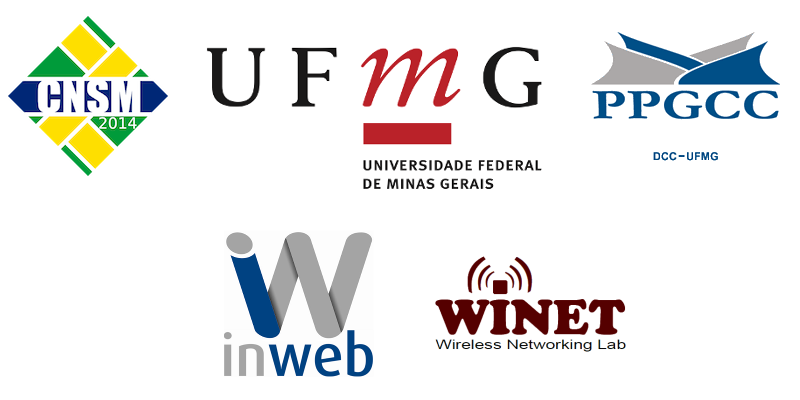
\includegraphics[width=\linewidth]{img/cnsm-footer.png}
    \end{figure}
\end{frame}


%
% Introduction
%
\begin{frame}\frametitle{Introduction - problem}

    \begin{itemize}
        \item SDN facilitates the network management 
        \item The interaction (API) with the Openflow switch is different on each
              controller
        \item Almost all applications need a topological view of the network
    \end{itemize}

\end{frame}


%
% Introduction
%
\begin{frame}\frametitle{Introduction - motivation}

    \begin{itemize}
        \item Provide an abstraction more close to the network
        \item Clarify network changes to the programmer
        \item Facilitate the network management
    \end{itemize}

\end{frame}


%
% Introduction
%
\begin{frame}\frametitle{Introduction - solution}

    \begin{itemize}
        \item Control plane representation in a graph model
        \item Real time control of network state
        \item Consistent and global topological view
        \item Base to other applications
    \end{itemize}

\end{frame}



%
% Controller
%
\begin{frame}\frametitle{Controller}

    \begin{itemize}
        \item We adopt POX, a Python-based, event-oriented controller
        \item Network elements are entities:
            \begin{itemize}
                \item Switch $\cdot$ Router $\cdot$ Host
            \end{itemize}
        \item The design is modular
        \item Experiments are simple and easy to run
    \end{itemize}

	\begin{figure}[h]
        \centering
        
\includegraphics[scale=0.2]{img/pox.png}
    \end{figure}
\end{frame}
